\section{Sobre los prototipos}

  Son un modelo o una muestra inicial de una pieza mecánica que se utiliza para probar y evaluar su diseño, funcionalidad y rendimiento antes de la producción en masa. Los prototipos permiten identificar posibles problemas, realizar ajustes y mejoras, y asegurar que la pieza cumpla con los requisitos y especificaciones deseadas. Según \cite{Christie2012}, los prototipos son esenciales en el proceso de desarrollo de productos, ya que facilitan la comunicación entre diseñadores, ingenieros y clientes, y ayudan a reducir costos y tiempos de producción al detectar errores en etapas tempranas.

  \subsection{¿Qué es el prototipo de un producto?}

  Un prototipo de un producto es una versión preliminar o modelo inicial que se crea para representar y probar las características, funcionalidades y diseño de un producto antes de su fabricación o producción en masa. Los prototipos pueden variar en complejidad, desde simples maquetas hasta modelos funcionales que simulan el comportamiento real del producto final.

  \subsection{¿Cuál es la utilidad del prototipo de un producto?}

  La utilidad del prototipo de un producto radica en varios aspectos:

  \begin{itemize}
    \item \textbf{Validación del diseño:} Permite evaluar y validar el diseño del producto, identificando posibles problemas o mejoras antes de la producción en masa.
    \item \textbf{Pruebas funcionales:} Facilita la realización de pruebas funcionales para verificar que el producto cumple con los requisitos y especificaciones deseadas.
    \item \textbf{Retroalimentación del usuario:} Proporciona una oportunidad para obtener retroalimentación de los usuarios o clientes potenciales, lo que puede ayudar a mejorar el diseño y la usabilidad del producto.
    \item \textbf{Reducción de costos:} Ayuda a identificar y corregir errores o problemas en una etapa temprana del desarrollo, lo que puede reducir los costos asociados con cambios posteriores en la producción.
  \end{itemize}

  \subsection{¿Qué objetivos se tienen al realizar el prototipo de un producto?}

  Al realizar el prototipo de un producto, se tienen varios objetivos clave:

  \begin{itemize}
    \item \textbf{Detección temprana de problemas:} Identificar y resolver problemas de diseño o funcionalidad antes de la producción en masa.
    \item \textbf{Mejora continua:} Utilizar la retroalimentación obtenida durante las pruebas del prototipo para realizar mejoras en el diseño y la funcionalidad del producto.
    \item \textbf{Alineación del equipo:} Facilitar la comunicación y la colaboración entre los diferentes miembros del equipo de desarrollo, asegurando que todos estén en la misma página.
    \item \textbf{Reducción de riesgos:} Minimizar los riesgos asociados con el lanzamiento de un nuevo producto al validar su diseño y funcionalidad antes de la producción.
  \end{itemize}

  \subsection{¿Qué materiales se utilizan para la elaboración de prototipos?}

  Dentro del contexto de piezas mecánicas, los materiales comúnmente utilizados para la elaboración de prototipos incluyen:

  \begin{itemize}
    \item \textbf{Plásticos:} Materiales como el acrílico, el poliestireno y el nylon son populares debido a su facilidad de moldeado y bajo costo.
    \item \textbf{Metales:} En algunos casos, se utilizan metales como el aluminio o el acero para prototipos que requieren mayor resistencia y durabilidad.
    \item \textbf{Espumas:} Las espumas de poliuretano o poliestireno se utilizan a menudo para crear prototipos ligeros y de bajo costo.
    \item \textbf{Resinas:} Las resinas epoxi o de poliéster se utilizan en la impresión 3D para crear prototipos con detalles precisos.
    \item \textbf{Madera:} La madera contrachapada o MDF se utiliza para prototipos que requieren un acabado estético o una estructura más robusta.
  \end{itemize}

  Finalmente, los prototipos de piezas mecánicas son esenciales para el desarrollo y la validación de nuevos productos, permitiendo a los ingenieros y diseñadores evaluar y mejorar sus diseños antes de la producción en masa. El uso de materiales adecuados y la realización de pruebas exhaustivas son fundamentales para garantizar el éxito del producto final \cite{Dym2013}.

  A continuación, se presentan los 5 prototipos de piezas mecánicas solicitadas:

  \newpage

  \section{Prototipo 1: Sólido en el primer octante.}

  Dado el sólido que se forma en el primer octante que tiene por vértices: $P(0,0,0)$, $P(13,0,0)$, $P(0,11,0)$, $P(0,0,19)$.
\vspace{-1cm}
  \begin{center}
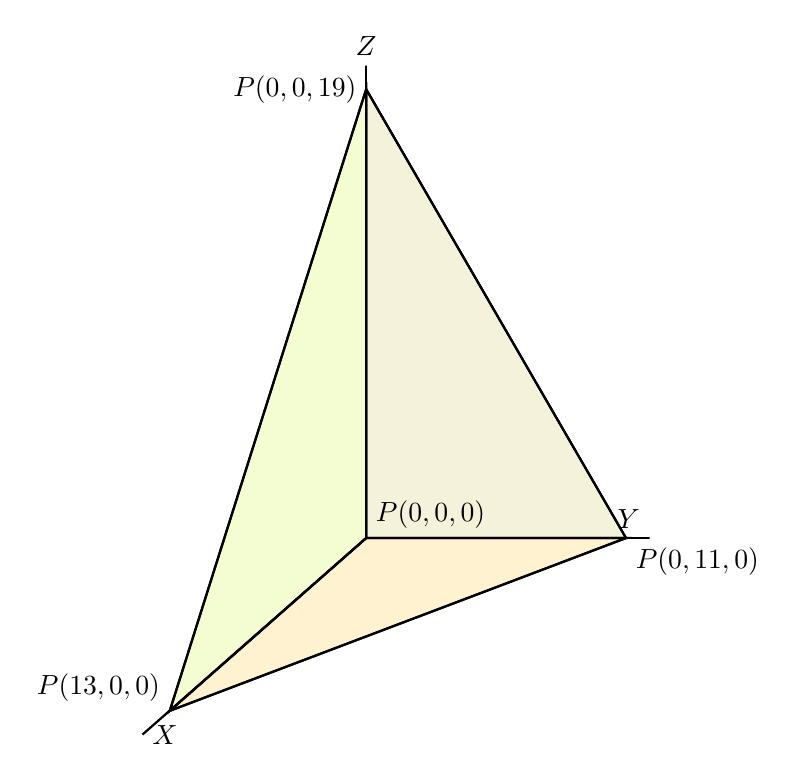
\begin{tikzpicture}[scale=0.3]
  % Definir coordenadas con perspectiva simple
  \coordinate (Z) at (0,20,0);
  \coordinate (Y) at (12,0,0);
  \coordinate (X) at (-1,0.15,22);
  \coordinate (O) at (0,0,0);
  \coordinate (A) at (11,0,0);
  \coordinate (B) at (0,19,0);  % Desplazado en x para perspectiva
  \coordinate (C) at (-1,0,19);   % Desplazado para mejor visualización

  % Caras del tetraedro
  \fill[blue!20, opacity=0.7] (O) -- (A) -- (B) -- cycle;
  \fill[red!20, opacity=0.7] (O) -- (A) -- (C) -- cycle;
  \fill[green!20, opacity=0.7] (O) -- (B) -- (C) -- cycle;
  \fill[yellow!20, opacity=0.7] (A) -- (B) -- (C) -- cycle;

  % Aristas
  \draw[thick] (O) -- (Z) -- cycle;
  \draw[thick] (O) -- (X) -- cycle;
  \draw[thick] (O) -- (Y) -- cycle;
  \draw[thick] (O) -- (A) -- (B) -- cycle;
  \draw[thick] (O) -- (A) -- (C) -- cycle;
  \draw[thick] (O) -- (B) -- (C) -- cycle;
  \draw[thick] (A) -- (B) -- (C) -- cycle;

  % Etiquetas
  \node[above] at (Z) {$Z$};
  \node[right] at (X) {$X$};
  \node[above left] at (Y) {$Y$};
  \node[above right] at (O) {$P(0,0,0)$};
  \node[below right] at (A) {$P(0,11,0)$};
  \node[left] at (B) {$P(0,0,19)$};
  \node[above left] at (C) {$P(13,0,0)$};
\end{tikzpicture}
\end{center}

\begin{multicols}{2}
\textbf{Representación de matemática de la superficie inclinada del sólido:}

Dado los puntos $P(13,0,0)$, $P(0,11,0)$ y $P(0,0,19)$. La ecuación del plano se puede expresar en forma intercepto como:

\[\frac{x}{13}+\frac{y}{11}+\frac{z}{19}=1\]

Luego por MCM:
\[19 \cdot 11 \cdot 13\ \Rightarrow 2717\]
\[19(11)x + 19(13)y + 11(13)z = 2717\]
\[209x + 247y + 143z = 2717\]
\[143z=2717-209x-247y\]
\[z=\frac{2717-209x-247y}{143}\]
\[f(x,y)=\frac{2717-209x-247y}{143}\]

\textbf{Cálculo de las áreas laterales del sólido:}

Área del plano A, región en el plano XZ:

\[\int_0^{13} \int_0^{\frac{-19}{13}x+19} dz\,dx = \int_0^{13} \left[ z \right]_0^{\frac{-19}{13}x+19} dx\]
\[\int_0^{13} \left( \frac{-19}{13}x+19 \right) dx = \left[ -\frac{19x^2}{26} + 19x \right]_0^{13}\]
\[-\frac{19(13)^2}{26} + 19(13) = \frac{247}{2} \approx 123.5\]

Área del plano A, región en el plano YZ:

\[\int_0^{11} \int_0^{\frac{-19}{11}y+19} dz\,dy = \int_0^{11} \left[ z \right]_0^{\frac{-19}{11}y+19} dy\]
\[\int_0^{11} \left( \frac{-19}{11}y+19 \right) dy = \left[ -\frac{19y^2}{22} + 19y \right]_0^{11}\]
\[-\frac{19(11)^2}{22} + 19(11) = \frac{209}{2} \approx 104.5\]

Área del plano A, región en el plano XY:

\[\int_0^{13} \int_0^{\frac{-11}{13}x+11} dy\,dx = \int_0^{13} \left[ y \right]_0^{\frac{-11}{13}x+11} dx\]
\[\int_0^{13} \left( \frac{-11}{13}x+11 \right) dx = \left[ -\frac{11x^2}{26} + 11x \right]_0^{13}\]
\[-\frac{11(13)^2}{26} + 11(13) = \frac{143}{2} \approx 71.5\]
\end{multicols}

\textbf{Cálculo del volúmen del sólido:}

De acuerdo a:

\[
V=\iint_{R} z(x,y)\,dA
\]

Entonces:

\[V=\int_0^{13} \int_0^{\frac{-11}{13}x+11} \left(\frac{2717-209x-247y}{143}\right) dy\,dx = \frac{1}{143} \int_0^{13} \int_0^{\frac{-11}{13}x+11} \left(2717-209x-247y\right) dy\,dx\]
\[V=\frac{1}{143} \int_0^{13} \left[ 2717y - 209xy - \frac{247y^2}{2} \right]_0^{\frac{-11}{13}x+11} dx\]
\[V=\frac{1}{143} \int_0^{13} \left( 2717\left(\frac{-11}{13}x+11\right) - 209x\left(\frac{-11}{13}x+11\right) - \frac{247\left(\frac{-11}{13}x+11\right)^2}{2} \right) dx\]
\[V=\frac{1}{143} \int_0^{13} \left(-\frac{29887}{13}x+29887+\frac{2299x^2}{13}-2299x-\frac{247}{2}\left(\frac{121}{169}x^2-\frac{242}{13}x+121\right)\right) dx\]
\[V=\frac{1}{143}\int_{0}^{13}\left(-\frac{777062}{338}x+\frac{10101806}{338}+\frac{59774}{338}x^2-\frac{777062}{338}x-\frac{29887}{338}x^{2}+\frac{777062}{338}x-\frac{5050903}{338}\right) dx\]
\[V=\frac{1}{143(338)} \int_{0}^{13} \left(-777062x+10101806+59774x^2-777062x-29887x^{2}+777062x-5050903\right) dx\]
\[V=\frac{1}{143(338)} \int_{0}^{13} \left(29887x^{2}-777062x+5050903\right) =\frac{1}{48334} \left[ \frac{29887x^{3}}{3} - \frac{777062x^{2}}{2} + 5050903x \right]_0^{13}dx\]
\[V=\frac{1}{48334} \left[ \frac{29887(13)^{3}}{3} - \frac{777062(13)^{2}}{2} + 5050903(13) \right] = \frac{1}{48334}\left(\frac{65661739}{3}-\frac{131323478}{2}+65661739\right)\]
\[V = \frac{2717}{6} \approx 452.8\ u^3\]

Conclusión: La aplicación del cálculo integral en la determinación del volumen y las áreas laterales son en fundamento iguales a las fórmulas geométricas tradicionales, sin embargo, el uso de integrales permite una mayor flexibilidad y precisión en la evaluación de sólidos con formas complejas o irregulares. Finalmente, es importante tener cuidado al momento de plantear los límites de integración ya que si bien por el teorema de Fubini se puede cambiar el orden de integración, los límites deben ser correctamente ajustados para reflejar la región de integración adecuada.

\newpage

\section{Prototipo 2: Centro de masa de una lámmina.}

El segundo prototipo debe ser diseñado como una lámina para proteger un dispositivo electrónico. Dicha lámina debe ser diseñada en un plano cartesiano limitada por los ejes coordenados del primer cuadrante y por la gráfica de la función:

\[f(x) = 14-x^{2}\]

Dada la fórmula para calcular el centro de masa de una lámina:
\[\bar{x} = \frac{\int_{a}^{b} xf(x) \, dx}{\int_{a}^{b} f(x) dx} \quad , \quad \bar{y} = \frac{\int_{a}^{b} \frac{f(x)^{2}}{2} \, dx}{\int_{a}^{b} f(x) dx} \]

\begin{multicols}{2}
  \textbf{Cálculo del área de la lámina:}
  \[\int_0^{\sqrt{14}} (14 - x^{2}) \, dx = \left[ 14x - \frac{x^{3}}{3} \right]_0^{\sqrt{14}}\]
  \[ = 14\sqrt{14} - \frac{(\sqrt{14})^{3}}{3} = \frac{28\sqrt{14}}{3} \approx 34.99\ u^{2}\]
  \textbf{Cálculo de $\bar{x}$:}
  \[\bar{x} = \int_0^{\sqrt{14}} x(14 - x^{2}) \, dx = \int_0^{\sqrt{14}}\left(14x-x^{3}\right)dx\]
  \[= \left[ 7x^{2} - \frac{x^{4}}{4} \right]_0^{\sqrt{14}} = 7(14) - \frac{(14)^{2}}{4} = 98 - 49 = 49\]
  \[\bar{x} = \frac{49}{\frac{28\sqrt{14}}{3}} = \frac{3\sqrt{14}}{8} \approx 1.4\]
  \textbf{Cálculo de $\bar{y}$:}
  \[\bar{y} = \int_0^{\sqrt{14}} \frac{(14 - x^{2})^{2}}{2} \, dx = \frac{1}{2}\int_0^{\sqrt{14}} 196 - 28x^{2} + x^{4} dx\]  
  \[= \frac{1}{2} \left[ 196x - \frac{28x^{3}}{3} + \frac{x^{5}}{5} \right]_0^{\sqrt{14}}\]
  \[=\frac{1}{2} \left( 196\sqrt{14} - \frac{28(\sqrt{14})^{3}}{3} + \frac{(\sqrt{14})^{5}}{5} \right)\]
  \[=98\sqrt{14} - \frac{14(\sqrt{14})^{3}}{3} + \frac{(\sqrt{14})^{5}}{10} \]
  \[\bar{y} = \frac{98\sqrt{14} - \frac{14(\sqrt{14})^{3}}{3} + \frac{(\sqrt{14})^{5}}{10}}{\frac{28\sqrt{14}}{3}} = \frac{28}{5} \approx 5.6\]
  \textbf{Finalmente:} Centroide de masa de la lámina:
  \[(\bar{x}, \bar{y}) = \left(\frac{3\sqrt{14}}{8}, \frac{28}{5}\right) \approx (1.4, 5.6)\]
\end{multicols}
\begin{center}
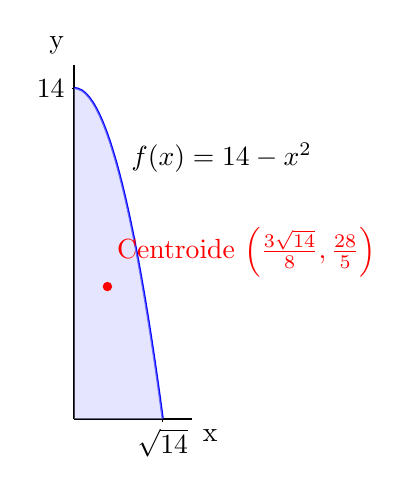
\begin{tikzpicture}[scale=0.3]
  % Ejes coordenados
  \draw[thick] (0,0) -- (5,0) node[anchor=north west] {x};
  \draw[thick] (0,0) -- (0,15) node[anchor=south east] {y};
  % Gráfica de la función f(x) = 14 - x^2
  \draw[domain=0:3.74, smooth, variable=\x, blue, thick] plot ({\x}, {14 - \x*\x});
  % Sombreado del área bajo la curva
  \fill[blue!20, opacity=0.5] (0,0) -- plot[domain=0:3.74, smooth, variable=\x] ({\x}, {14 - \x*\x}) -- (3.74,0) -- cycle;
  % Punto del centroide
  \fill[red] (1.4, 5.6) circle (0.2) node[anchor=south west] {Centroide $\left(\frac{3\sqrt{14}}{8}, \frac{28}{5}\right)$};
  % Marcar interceptos
  \draw (3.74,0) -- ++(0,-0.12); % muesca en eje x
  \draw (0,14) -- ++(-0.12,0);   % muesca en eje y
  \node[below] at (3.74,0) {$\sqrt{14}$};
  \node[left]  at (0,14)   {$14$};
  % Etiqueta de la función
  \node[above right] at (2,10) {$f(x) = 14 - x^{2}$};
\end{tikzpicture}
\end{center}
\textbf{Conclusión:} El cálculo del centro de masa de una lámina utilizando integrales puede verse como una media ponderada de las coordenadas, donde la función que define la lámina actúa como el peso o densidad en cada punto. Este enfoque es especialmente útil para láminas con formas irregulares, donde las fórmulas geométricas tradicionales no son aplicables. Además, el uso de integrales permite una mayor precisión y flexibilidad en la evaluación de diferentes formas y distribuciones de masa.

\newpage

\section{Prototipo 3: Región entre dos curvas.}

El cuarto prototipo debe ser una placa metálica (lámina), la cual se diseña como la región encerrada por las gráficas de $f(x)=2\sqrt{x}$ y $g(x)=\frac{x}{2}$.

\begin{center}
\begin{tikzpicture}[scale=0.35]
  % ejes
  \draw[thick] (-0.5,0) -- (18,0) node[right] {x};
  \draw[thick] (0,-0.5) -- (0,10) node[above] {y};

  % marcas
  \foreach \x in {0,4,8,12,16} \draw (\x,0.12) -- (\x,-0.12) node[below] {\x};
  \foreach \y in {0,2,4,6,8}  \draw (0.12,\y) -- (-0.12,\y) node[left] {\y};

  % región sombreada entre curvas (de 0 a 16, intersección en x=16)
  \fill[green!30,opacity=0.5]
    plot[domain=0:16,smooth,variable=\x] ({\x},{2*sqrt(\x)})
    -- plot[domain=16:0,smooth,variable=\x] ({\x},{\x/2})
    -- cycle;

  % curvas
  \draw[domain=0:16,smooth,variable=\x,blue,thick]
    plot ({\x},{2*sqrt(\x)})
    node[xshift=-100pt, yshift=-15pt] {$y=2\sqrt{x}$};
  \draw[domain=0:16,smooth,variable=\x,red,thick]  plot ({\x},{\x/2})       node[xshift=-80pt, yshift=-55pt] {$y=\tfrac{x}{2}$};

  % puntos de intersección
  \fill (0,0) circle (2pt) node[below left] {$(0,0)$};
  \fill (16,8) circle (2pt) node[above right] {$(16,8)$};
\end{tikzpicture}
\end{center}

\begin{multicols}{2}
  \textbf{Cálculo de los puntos en común:}
  Para encontrar los puntos en común entre las dos curvas, se igualan las funciones:
  \[2\sqrt{x} = \frac{x}{2}\]
  \[4\sqrt{x} = x\]
  \[16x = x^{2}\]
  \[x^{2} - 16x = 0\]
  \[x(x - 16) = 0\]
  \[x = 0 \quad \land \quad x = 16\]

  \textbf{Cálculo del área de la región:}
  El área de la región encerrada entre las dos curvas se calcula mediante la integral definida:
  \[A = \int_0^{16} \int_{\frac{x}{2}}^{2\sqrt{x}} dy \, dx = \int_0^{16} \left[ y \right]_{\frac{x}{2}}^{2\sqrt{x}} dx\]
  \[A = \int_0^{16} \left( 2\sqrt{x} - \frac{x}{2} \right) dx = \left[ \frac{4}{3}x^{\frac{3}{2}} - \frac{x^{2}}{4} \right]_0^{16}\]
  \[A = \left( \frac{4}{3}(16)^{\frac{3}{2}} - \frac{(16)^{2}}{4} \right) - \left( 0 \right)\]
  \[A = \left( \frac{4}{3}(64) - 64 \right) = \frac{256}{3} - 64 = \frac{256 - 192}{3} = \frac{64}{3}\]
  \[\approx 21.33\ u^{2}\]
  
  \textbf{Cálculo del perímetro de la región:}
  El perímetro de la región se calcula sumando las longitudes de las curvas y los segmentos de línea que forman el borde de la región:
  \[P = \int_0^{16} \sqrt{1 + \left( \frac{d}{dx}(2\sqrt{x}) \right)^{2}} + \sqrt{1 + \left( \frac{d}{dx}\left(\frac{x}{2}\right) \right)^{2}} \, dx\]
  \[P = \int_0^{16} \sqrt{1 + \left( \frac{1}{\sqrt{x}} \right)^{2}} + \sqrt{1 + \left( \frac{1}{2} \right)^{2}} \, dx\]
  \[P = \int_0^{16} \sqrt{1 + \frac{1}{x}} + \int_{0}^{16}\sqrt{1 + \frac{1}{4}} \, dx\]
  \[P = 18.5871 + \int_{0}^{16}\sqrt{1 + \frac{1}{4}} \, dx\]
  \[P = 18.5871 + \int_{0}^{16}\frac{\sqrt{5}}{2} \, dx\]
  \[P = 18.5871 + \left[ \frac{\sqrt{5}}{2}x \right]_0^{16} = 18.5871 + 8\sqrt{5} \approx 36.36\ u\]

  \textbf{Se propone la siguiente densidad proporcional al eje x:}
  \[\rho(x) = 2x\] 
  Por lo tanto:
  \[\rho=\frac{m}{A} \implies m = \rho A\]
  \textbf{Cálculo de la masa de la lámina:}
  \[m= \rho (x)\iint_R \, dA \implies \iint_R \rho (x) \, dA\]
  \[m = \int_0^{16} \int_{\frac{x}{2}}^{2\sqrt{x}} 2x \, dy \, dx = \int_0^{16} \left[ 2xy \right]_{\frac{x}{2}}^{2\sqrt{x}} dx\]
  \[=\int_0^{16} \left( 2x(2\sqrt{x}) - 2x\left(\frac{x}{2}\right) \right) dx = \int_0^{16} \left( 4x^{\frac{3}{2}} - x^{2} \right) dx\]
  \[= \left[ \frac{8}{5}x^{\frac{5}{2}} - \frac{x^{3}}{3} \right]_0^{16} = \left( \frac{8}{5}(16)^{\frac{5}{2}} - \frac{(16)^{3}}{3} \right) - (0)=\]
  \[m = \left( \frac{8}{5}(1024) - \frac{4096}{3} \right) = \frac{4096}{15} \approx 273.07\ g\]
\end{multicols}

\textbf{Conclusión:} El cálculo del área, perímetro y masa de una lámina definida por la región entre dos curvas utilizando integrales es útil para evaluar propiedades físicas y geométricas de objetos con formas irregulares. Se esocogió una densidad variable para ilustrar cómo la masa puede depender de la posición dentro de la lámina, lo que es relevante en aplicaciones prácticas donde la distribución de masa no es uniforme.

\section{Conclusión general}

En conclusión, herramientas como la integral, integral doble, integral de longitud de arco y centroide se basan en principios matemáticos geométricos fundamentales. Estas herramientas permiten analizar y resolver problemas complejos relacionados con áreas, volúmenes, longitudes y distribuciones de masa en diversas aplicaciones de ingeniería y diseño de piezas mecánicas. Al comprender y aplicar estos conceptos, los ingenieros pueden optimizar diseños, mejorar la funcionalidad y garantizar la eficiencia en la fabricación de componentes mecánicos.
